\documentclass{include/thesisclass}
\usepackage{esvect}
\usepackage{amsthm}
\usepackage{listings}
\lstset{language=java}
\usepackage{hyperref}
\usepackage[ngerman]{babel}
% Main File - Based on thesisclass.cls
% Comments are mostly in English
% ------------------------------------------------------------------------------
% Further files in folder:
%  - include/cmds.tex (for macros and additional commands)
%  - include/kitlogo.pdf (for titlepage)
%  - lit.bib (bibtex bibliography database)
%  - include/titlepage.tex (for layout of titelpage)
% ------------------------------------------------------------------------------
% Useful Supplied Packages:
% amsmath, amssymb, mathtools, bbm, upgreek, nicefrac,
% siunitx, varioref, booktabs, graphicx, tikz, multicol





%% -------------------------
%% |    Thesis Settings    |
%% -------------------------
% english or ngerman (new german für neue deutsche Rechtschreibung statt german)
\SelectLanguage{ngerman}
% details on this thesis
\newcommand{\thesisauthor}{Kiril Voigtländer}
\newcommand{\thesistopic}{Name des Themas auf Deutsch}
\newcommand{\thesisentopic}{Name of the Topic in English}
\newcommand{\thesislongtopic}{Very long and very detailed description of the very interesting thesis topic (only necessary for pdfsubject tag).}
\newcommand{\thesisinstitute}{Otto-Kühne-Schule}
\newcommand{\thesisreviewerone}{Herr Schmalstieg}
\newcommand{\thesisreviewertwo}{}
\newcommand{\thesisadvisorone}{} % to use: enter names and uncomment in titlepg
\newcommand{\thesisadvisortwo}{}
\newcommand{\thesistimestart}{01.04.2015} % on titlepage
\newcommand{\thesistimeend}{30.09.2015} % on titlepage
\newcommand{\thesistimehandin}{30.09.2015} % on second page 'preamble'
\newcommand{\thesispagehead}{Facharbeit: \thesisentopic} % page heading
% eigene Befehlsdefinitionen:
\newcommand{\vektor}[3]{\left(\begin{array}{c}#1\\#2\\#3\end{array}\right)}
\newcommand{\m}[9]{\left(\begin{array}{ccc}
#1&#2&#3\\
#4&#5&#6\\
#7&#8&#9\\
\end{array}\right)}




%% ---------------------
%% |    PDF - Setup    |
%% ---------------------
% This information will appear embed into the PDF file as meta data, but will 
% not be printed anywhere
\hypersetup
{
    pdfauthor={\thesisauthor},
    pdftitle={Bachelorarbeit: \thesistopic},
    pdfsubject={\thesislongtopic},
    pdfkeywords={kit,physik,bachelor,thesis,\thesisauthor}
}





%% --------------------------------------
%% |    Settings for Word Separation    |
%% --------------------------------------
% Help for separation:
% In German package the following hints are additionally available:
% "- = Additional separation
% "| = Suppress ligation and possible separation (e.g. Schaf"|fell)
% "~ = Hyphenation without separation (e.g. bergauf und "~ab)
% "= = Hyphenation with separation before and after
% "" = Separation without a hyphenation (e.g. und/""oder)

% Describe separation hints here:
\hyphenation
{
    über-nom-me-nen an-ge-ge-be-nen
    %Pro-to-koll-in-stan-zen
    %Ma-na-ge-ment  Netz-werk-ele-men-ten
    %Netz-werk Netz-werk-re-ser-vie-rung
    %Netz-werk-adap-ter Fein-ju-stier-ung
    %Da-ten-strom-spe-zi-fi-ka-tion Pa-ket-rumpf
    %Kon-troll-in-stanz
}





%% -----------------------
%% |    Main Document    |
%% -----------------------
\usepackage{lipsum} % for Lorem Ipsum text example
\begin{document}
    % Titlepage and ToC
    \FrontMatter

    % coordinates for background border
\newcommand{\diameter}{20}
\newcommand{\xone}{-15}
\newcommand{\xtwo}{160}
\newcommand{\yone}{15}
\newcommand{\ytwo}{-253}




\begin{titlepage}
    % background border
    \begin{tikzpicture}[overlay]
    \draw[color=gray]
            (\xone mm, \yone mm)
      -- (\xtwo mm, \yone mm)
    arc (90:0:\diameter pt)
      -- (\xtwo mm + \diameter pt , \ytwo mm)
        -- (\xone mm + \diameter pt , \ytwo mm)
    arc (270:180:\diameter pt)
        -- (\xone mm, \yone mm);
    \end{tikzpicture}



    % KIT image and sign for faculty of physics
    \begin{textblock}{10}[0,0](4.5,2)
         \includegraphics[width=.25\textwidth]{include/PädaLogo.pdf}
    \end{textblock}
    \changefont{phv}{m}{n}    % helvetica
    \begin{textblock}{10}[0,0](5.5,2.2)
        \begin{flushright}
            \Large Leistungskurs PHYSIK\\\thesisinstitute
        \end{flushright}
    \end{textblock}



    % horizontal line
    \begin{textblock}{10}[0,0](4.2,3.1)
        \begin{tikzpicture}[overlay]
        \draw[color=gray]
                (\xone mm + 5 mm, -12 mm)
          -- (\xtwo mm + \diameter pt - 5 mm, -12 mm);
        \end{tikzpicture}
    \end{textblock}



    % begin of text part
    \changefont{phv}{m}{n}    % helvetica
    \centering



    % thesis topic (en and ge)
    \vspace*{3cm}
    \Huge\thesistopic\\
    \huge(\thesisentopic)\\



    % author name and institute
    \vspace*{2cm}
    \Large Facharbeit\\von\\
    \vspace*{1cm}
    \huge\thesisauthor\\
    \vspace*{1cm}
    \Large an der \thesisinstitute



    % possible frontimage - thanks to JabberWok
    % for publishing the img under GNU Document License
    \vspace*{1.5cm}
    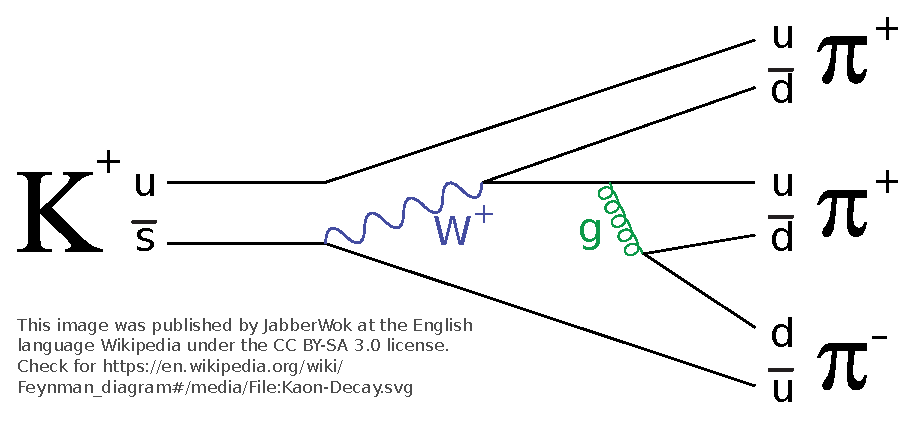
\includegraphics[scale=0.7]{./include/frontimage.eps}\\



    % examiners (Referenten)
    \vspace*{1.5cm}
    \Large
    \begin{center}
        \begin{tabular}[ht]{l c l}
        \iflanguage{english}{Reviewer}{Referent}: 
            & \hfill & \thesisreviewerone\\
        \iflanguage{english}{Second Reviewer}{Korreferent}: 
            & \hfill & \thesisreviewertwo\\
        % uncomment if you want to provide info on your advisors
        %\iflanguage{english}{Advisor}{Betreuender Mitarbeiter}: 
        %    & \hfill & \thesisadvisorone\\
        %\iflanguage{english}{Second Advisor}{Zweiter betreuender Mitarbeiter}: 
        %    & \hfill & \thesisadvisortwo\\
        \end{tabular}
    \end{center}



    % working time
    \vspace{1cm}
    \begin{center}
        \large{{Bearbeitungszeit}: \thesistimestart \hspace*{0.25cm} -- %
                                   \hspace*{0.25cm} \thesistimeend}
    \end{center}



    % lowest text blocks concerning the KIT
    \begin{textblock}{10}[0,0](4,16.8)
        \tiny{PÄDA -- Otto-Kühne-Schule}
    \end{textblock}
    \begin{textblock}{10}[0,0](14,16.75)
        \large{\textbf{www.kit.edu}}
    \end{textblock}
\end{titlepage}

    \chapter*{Erklärung zur Selbstständigkeit}
Ich versichere, dass ich diese Arbeit selbstständig verfasst habe und keine %
anderen als die angegebenen Quellen und Hilfsmittel benutzt habe, die %
wörtlich oder inhaltlich übernommenen Stellen als solche kenntlich gemacht habe. %und %
%die Satzung des KIT zur Sicherung guter wissenschaftlicher Praxis in der %
%gültigen Fassung vom 17.05.2010 beachtet habe.\\

\vspace{1cm}

\renewcommand{\arraystretch}{0} % for spacing in the tabular environment

\begin{flushright}
	\begin{tabular}{rr}
		Bonn, den \thesistimehandin, & \hspace*{5cm}\\[0mm]
		\cline{2-2}\\[2mm]    % the last line has height 2mm due
		& \thesisauthor       % to \arraystretch=0
	\end{tabular}
\end{flushright}

\vfill

\begin{flushright}
	Als Ansichtsexemplar genehmigt von\\
	\vspace{1cm}
	\begin{tabular}{rr}
		Bonn, den \thesistimehandin, & \hspace*{5cm}\\[0mm]
		\cline{2-2}\\[2mm]    % the last line has height 2mm due
		& \thesisreviewerone  % to \arraystretch=0
	\end{tabular}
\end{flushright}

\renewcommand{\arraystretch}{1}

%\cleardoublepage


    \begingroup \let\clearpage\relax    % in order to avoid listoffigures and
    \tableofcontents                    % listoftables on new pages
    \listoffigures
    \listoftables
    \endgroup
    \cleardoublepage



    % Contents
    \MainMatter

    \chapter{Einleitung}
    \label{chap:Einleitung}
    Die vorliegende Facharbeit befasst sich mit dem Modell des Röhrenfernsehers.
Röhrenfernseher sind Geräte, bei welchen ein Bild durch entweder einer elektrischen oder einer magnetischen Ablenkung auf einen Bildschirm gelenkt werden.
Des Weiteren wird der Röhrenfernseher in der dazu gelegten Animation bildlich dargestellt.
Sowohl die Animation als auch ihre physikalischen Eigenschaften werden in dem Kapitel \ref{chap:sim} erläutert.
Im ersten Kapitel nach der Einleitung wird die Theorie des E-Feldes und des B-Feldes betrachtet.
Für das E-Feld wichtig ist, dass es eine Ladung gibt, da um jede Ladung ein elektrisches Feld gibt.
Des Weiteren wird die Herleitung der Coulombkraft betrachtet.
Anschließend folgt eine genauere Betrachtung eines Plattenkondensators, welcher einen Spezialfall eines elektrischen Feldes darstellt.
Dabei wird auf die Formel für die Kapazität "`$C$"' und für die gespeicherte Energie im Plattenkondensator betrachtet.
Dies geschieht im Kapitel \ref{sec:Plattenkondensator}.
Für das B-Feld ist der Magnetismus wichtig, welcher zu der Entstehung des B-Feldes führt.
Hier wird die Herleitung der Lorentzkraft getätigt.
Anschließend folgt eine genauere Betrachtung des Fadenstrahlrohrs, welcher zur der Bestimmung der spezifischen Ladung "`$\frac{e}{m}$"' benutzt wird.
Diese Betrachtung geschieht im Kapitel \ref{sec:Fadenstrahlrohr}.
Des Weiteren wird die Wechselwirkung der beiden Felder aufeinander betrachtet.
%genauer erklären was passiert. geht erst nach der stunde mit dem tutor und nachdem schreiben des Kapitels
Dies geschieht im Kapitel \ref{sec:Maxwell}.
Das folgende Kapitel \ref{chap:fern} ist in zwei Unterkapitel aufgeteilt.
Im ersten Unterkapitel \ref{sec:aufbau} wird der Aufbau der Fernsehröhre betrachtet.
Dabei ist wichtig zu beachten, dass ein Röhrenfernseher aus einer Einrichtung besteht, welche die Elektronen emittiert, einer Einrichtung, welche die Elektronen steuert, eine Einrichtung, welche die Elektronen ablenkt und ein Bildschirm, wo die Elektronen als Strahl auf einen Punkt treffen, wo das Bild erzeugt wird.
Die Ablenkung kann sowohl magnetisch als auch elektrisch sein.
Die Funktionsweise der Fernsehröhre wird im Kapitel \ref{sec:Funktionsweise} behandelt.
In diesem Kapitel wird des Weiteren auch erklärt, welche Kräfte auf das jeweilige Elektron in der jeweiligen Einrichtung wirken und welche Resultate dies mit sich zieht.
Als nächstes wird die Umsetzung der Fernsehröhre in die Animation betrachtet.
Dafür wird der Code der Animation betrachtet und erläutert.
Des Weiteren ist stets eine physikalische Erläuterung dabei, welche die Prozesse beschreibt die in der jeweiligen Einrichtung geschehen.

    \chapter{Theoretischer Hintergrund}
    \label{chap:Theorie}
    \section{E-Feld:}
\subsection{Entstehung und Beschreibung}
Jede Ladung wird von einem elektrischen Feld umgeben.
Zuerst muss der Begriff von Ladung geklärt werden:
Ladung ist eine Eigenschaft von Materie.
Die Einheit der Ladung ist 1$C$ (Coulomb).
Alle bisherigen Experimente legen nahe, dass es nur 2 Arten von elektrischer Ladung gibt; Positiv und Negativ.
Die Richtung der Feldlinien ist immer die Richtung der Kraftwirkung auf einen positiv geladenen Probekörper.
Eine Ladung bewirkt eine Kraft auf eine andere Ladung.
Gleich geladene Ladungen stoßen sich ab, während entgegengesetzte geladene Ladungen sich anziehen.
Diese Kraft wird als elektrische Kraft bezeichnet oder genauer als Coulomb-Kraft.
Die Herleitung der Coulomb-Kraft sieht wie folgt aus:
Man nehme sich zwei Punktladungen, welche mit $q_1$ und mit $q_2$ gekennzeichnet werden. 
Des Weiteren ist ein Abstand $r$ zwischen den Ladungen vorhanden.
Es gibt einmal die Kraft von $q_1$ auf $q_2$ ($\vv{F_{12}}$) und einmal die Kraft von $q_2$ auf $q_1$ ($\vv{F_{21}}$).
Durch betrachten der Formel: $F_{el} = \frac{q_1 \cdot q_2}{r^2}$ 
lässt sich schließen, dass wenn $r$ gleich bleibt, aber die die Ladungen $q_1$ und $q_2$ erhöht werden, die Coulomb-Kraft ebenfalls zunimmt.
Daraus lässt sich schließen, dass die elektrische Kraft proportional zu den Ladungen $q_1$ und $q_2$ ist. 
Wenn die Ladungen $q_1$ und $q_2$ gleich bleiben und $r$ erhöht wird, dann verringert sich die elektrische Kraft.
Daraus lässt sich wiederum schließen, dass die elektrische Kraft anti proportional zum Abstand $r$ ist.
Diese zuvor beschriebene Kraftwirkung, lässt sich mittels Probeladungen im ganzen Raum um die Ladung messen und als Vektor an jedem Punkt visualisieren.
Diese Visualisierung des Raumes nennt man elektrisches Feld.
Die jeweilige Stärke ergibt sich aus der Größe der Probeladung "`$q$"' und der Größe der Kraft "`$F_{el}$"' auf die Ladung.
Die Formel für das E-Feld ist : $E = \frac{F_{el}}{q}$.
Die Dimension des E-Feldes lautet: $[E] = \frac{N}{C} = \frac{V}{m}$.
Veranschaulichen lässt sich dies durch die Animation \cite{Animation}.

%Beschreibung
Wenn ein elektrisches Feld vorhanden ist, lässt sich dieses als Eigenschaft des Raums auffassen.
Die Kraftwirkung des elektrischen Feldes wird mit Probeladung ermittelt und durch Feldlinien visuell dargestellt.
Die Feldlinien kreuzen und berühren sich nicht.
Wenn die Feldlinien eng beieinander liegen (hohe Dichte), dann ist das dort existierende elektrische Feld stark.
Wenn die Dichte der Feldlinien allerdings niedrig ist, dann ist das elektrische Feld schwach.
Es gibt zwei unterschiedliche Arten von elektrischen Feldern. 
Es gibt zum einen das homogene elektrische Feld und zum anderen das inhomogene elektrische Feld.
Bei dem homogenen elektrischen Feld stehen die Feldlinien parallel zu einander und das elektrische Feld ist an allen Stellen gleich stark.
Bei dem inhomogenen elektrischen Feld kann diese Annahme nicht getätigt werden.
% hier eventuell noch auf die verschiedene Ladungen eingehen (Punktladung, etc.)
\subsection{Anwendung}
\label{sec:Plattenkondensator}
Als Anwendungsbeispiel lässt sich der Plattenkondensator nehmen:
Hier lässt sich die Annahme treffen, dass das elektrische Feld zwischen den Platten homogen ist.
Allerdings muss beachtet werden, dass diese Aussage nur zwischen den Platten des Kondensators gilt und das sobald man an die Ränder des Kondensators geht, diese Aussage wegbricht.
An den Rändern wirkt nämlich ein inhomogenes elektrisches Feld.
Des Weiteren ist das elektrische Feld als $E = \frac{U}{d}$ definiert.
Somit nimmt das elektrische bei einer größeren Spannung "`U"' zu und bei größerem Abstand der Platten "`d"' ab.
Beim Kondensator kann noch eine weitere Größe eingeführt werden, die Kapazität "`C"'.
Die Kapazität ist dabei so definiert, dass sie die maximale Menge an Ladung, die der Kondensator auf den Platten speichern kann, angibt.
Die Herleitung ist wie folgt:
$\mbox{Flächenladungsdichte: } \sigma \mbox{:=} \frac{Q}{A}$.
Dies führt zum elektrischen Feld mit $\sigma = \epsilon_0 \cdot E$ als Feldgleichung.
Dabei beträgt $\epsilon_0 = 8.854 \cdot 10^{-12} \frac{As}{Vm}$ und ist unter dem Namen "`Dielektrizitätskonstante"' bekannt.
Im allgemeinen ist das Feld auch noch vom jeweiligen Material abhängig, wodurch die Gleichung einen weiteren Term "`$\epsilon_r$"'enthält "`$\sigma = \epsilon_0 \cdot \epsilon_r \cdot E$ "'.
Diese zusätzliche Konstante berücksichtigt dabei die spezifische Materialeigenschaften und nennt sich "` relative Permeabilität"'.
Im Vakuum ist diese jedoch = 1.
Daraus folgt, dass $ Q = \epsilon_0 \cdot \epsilon_r \cdot \frac{A}{d} \cdot U$ ist.
Die Kapazität ist als $\mbox{C:= } \frac{Q}{U} = \epsilon_0 \cdot \epsilon_r \cdot \frac{A}{d}$ definiert.
Des Weiteren kann die Energie im Plattenkondensator bestimmt werden.
Dafür wird angenommen, dass der Kondensator zuerst neutral ist und eine äußere Spannung $U_0$ anliegt.
Im ersten Schritt fließt eine kleine Portion Ladung $\Delta Q$ mit dem Energieaufwand $\Delta W_1$ auf die andere Platte. Dabei entsteht die Spannung $U_1$ zwischen den Platten $\rightarrow$ $\Delta W_1 = U_1 \cdot \Delta Q$.
Es wird mehr Energie benötigt, um  weitere gleichgroße Ladungsportionen $\Delta Q$ auf die Platte zu bringen $\Delta W_2 = U_2 \cdot \Delta Q$.
Die letzte Ladungsportion $\Delta Q$ wird mit der Energie $\Delta W_E$ auf die Platte transportiert und dabei liegt zwischen den Platten die Spannung $U_0$ an. 
$\Delta W_E = U_0 \cdot \Delta Q$.
Daraus folgt die Gesamtenergie: W = $\Delta W_1 + \Delta W_2 +...+ \Delta W_E$
$$\Rightarrow W \mbox{ = } \frac{1}{2}\cdot Q_E \cdot U_o \mbox{ wegen $Q_E = C \cdot U_0$}$$
$$W= \frac{1}{2} \cdot C \cdot U_o^2$$
\section{B-Feld:}
\subsection{Entstehung und Beschreibung}
Als Grundlage, dass ein B-Feld entsteht muss der Magnetismus als Grundlage genommen werden.
Dafür muss der Begriff des Magnetismus zu erst geklärt werden.
Ein Magnet wird dadurch Entmagnetisiert, dass er gestoßen oder mit einer Temperatur oberhalb der Curie-Temperatur erhitzt wird $~600°C$.
Des Weiteren führt das Durchbrechen eines Magneten in der Mitte, dazu das zwei neue Magneten entstehen, es gibt keine magnetische Monopole.
Die Feldlinien eines Magneten verlaufen vom Nordpol zum Südpol.
Ein Magnetfeld bewirkt eine Kraft auf ein geladenes Teilchen.
Die wirkende Kraft wird als magnetische Kraft bezeichnet oder als Lorentzkraft, wenn es sich um einen einzelnen Ladungsträger handelt.
Die Herleitung der Lorentzkraft sieht wie folgt aus:
Man nehme sich einen Ladungsträger (negativ) und einen langen Leiter.
Die Formel für die magnetische Kraft lautet: $F_{mag} =  B \cdot I_L \cdot \Delta l$.
Der Strom $I_L$ kann durch $\frac{\Delta Q}{\Delta t}$ ersetzt werden.
Dadurch kommt die Formel $F_{mag} = B \cdot \frac{\Delta Q}{\Delta t} \cdot l$ raus. 
Als nächstes lässt sich $\Delta Q$ durch $N \cdot e$ ersetzten.
Dies führt zu der Formel $F_{mag} = B \cdot N \cdot e \cdot \frac{\Delta l}{\Delta t}$.
Dabei lässt sich der Quotient als $v$ vereinfachen, was die Geschwindigkeit der Ladungsträger angibt.
Dadurch beträgt die Formel für die magnetische Kraft nun: $F_{mag} = B \cdot N \cdot e \cdot v$.
Allerdings soll die Lorentzkraft hergeleitet werden, welches die Kraft auf einen einzelnen Ladungsträger darstellt, weshalb die magnetische Kraft mit $N$ dividiert werden muss.
Dies führt dazu, dass die Formel für die Lorentzkraft $F_L = B \cdot e \cdot v$ ist.
Diese Formel lässt sich für jede beliebige Ladung benutzen, weshalb $e$ durch $q$ ersetzt werden kann.
Daraus ergibt sich die Formel: $F_L = q \cdot B \cdot v$.
Der Vektor der Lorentzkraft senkrecht auf der durch den Geschwindigkeitsvektor und dem Vektor der Flussdichte aufgespannten Ebene \cite{Lorentzkraft}.
Magnetfelder entstehen in der Gegenwart von Dauermagneten (bestehend aus Eisen, Kobalt, Nickel oder Legierungen) oder in der Umgebung von stromdurchflossenen Leitern. 
Die Größe der magnetischen Flussdichte "`B"' ist den magnetischen Feldlinien zugeordnet.
Sie ist durch die Kraft definiert, welche ein stromdurchflossener Leiter erfährt.
Die Visualisierung des Raums nennt man magnetisches Feld.
Die jeweilige Stärke ergibt sich aus der Größe der Kraft "`$F_L$"', der Länge des Leiters "`$l$"' und der Stärke des elektrischen Stroms "`$I$"'.
Die Formel für das B-Feldd ist : $B = \frac{F_L}{I \cdot l}$.
Die Dimension des B-Feldes lautet: $[B] = \frac{N}{Am} = \frac{Vs}{m^2} = T$.

% Beschreibung von B-Feld
Wenn ein magnetisches Feld vorhanden ist, lässt sich dieses als Eigenschaft des Raums auffassen.
Die Kraftwirkung des magnetischen Feldes wird durch geladen Teilchen (Ladungen) ermittelt und durch Feldlinien visuell dargestellt.
Die Feldlinien kreuzen und berühren sich nicht.
Des Weiteren haben Sie keinen Anfangspunkt und kein Endpunkt, sondern sind stets geschlossen.
Wenn die Dichte an Feldlinien groß ist, dann ist die Magnetfeldstärke dementsprechend ebenfalls stark.
Wenn die Dichte an Feldlinien gering ist, dann ist die Magnetfeldstärke ebenfalls gering.
Es gibt verschiedene Magnete mit dementsprechend auch verschiedene Magnetfeldern. 
Zum einen liegt der Stabmagnet vor, bei welchem das magnetische Feld analog zum elektrischen Feld eines Dipols ist.
Zum anderen liegt der Hufeisenmagnet vor, welcher gleich wie der Plattenkondensator abgebaut ist.
Bei diesem ist das magnetische Feld im inneren homogen und an den Rändern inhomogen. 
\subsection{Anwendung}
\label{sec:Fadenstrahlrohr}
Als Anwendungsbeispiel lässt sich der Fadenstrahlrohr nehmen.
Hier lässt sich die Annahme treffen, dass das magnetische Feld im inneren der Helmholtz-Spule homogen ist. Des Weitern gelangen die betrachteten Elektronen mit einer Geschwindigkeit von $v=\sqrt{\frac{2 \cdot e \cdot U_B}{m}}$. Die Elektronen wurden davor in der Elektronenkanone freigesetzt.
Dies ist in dem Kapitel \ref{sec:tolle-section} bereits dargestellt. 
Der Fadenstrahlrohr kann dafür verwendet werden um die spezifische Ladung "`$\frac{e}{m}$"' eines Elektrons oder eines Ions zu bestimmen.
Dafür kann man durch die Linke-Hand-Regel die Ablenkung eines einzelnes Elektrons im Magnetfeld bestimmen. Dabei zeigt der Daumen, die Richtung der negativen Ladungsträger an, der Zeigefinger die Richtung der Feldlinien und der Mittelfinger die senkrecht dazu wirkende Lorentzkraft.
Wenn man dies nun anwendet, kommt man zu den Schluss, dass die Elektronen auf einer Kreisbahn abgelenkt werden. 
Dadurch wirkt die Lorentzkraft als Zentripetalkraft und kann gleich gesetzt werden.
$$F_L = F_z$$
$$e \cdot v \cdot B = \frac{m \cdot v^2}{r}$$
Diese Formel lässt sich als erstes durch $v$ dividieren und als Ergebnis kommt $e \cdot B = \frac{m \cdot v}{r}$.
Als nächste wird $v$ durch den oben genannten Wert %Verweis möglich?
ersetzt: $e \cdot B = m \cdot \frac{\sqrt{\frac{2 \cdot e \cdot U_B}{m}}}{r}$.
Nun lässt sich dieses Ergebnis quadrieren und durch $e$ dividieren: $e \cdot B^2 = m \cdot \frac{2 \cdot U_B}{r^2}$.
Als letztes kann die Gleichung noch durch $m$ und durch $B^2$ dividieren und als Ergebnis kommt für die spezifische Ladung "`$\frac{e}{m}$"' raus : $\frac{e}{m} = \frac{2 \cdot U_B}{ r^2 \cdot B^2}$.
Diese Formel gibt die spezifische Ladung eines Elektrons an, allerdings kann man $e$ auch durch $q$ ersetzten und dadurch die spezifische Ladung eines jeden anderen Ions berechnen.
\section{Wechselwirkung der Felder}%Maxwellgleichung
\label{sec:Maxwell}
Das folgende Kapitel bezieht sich hauptsächlich auf die Quelle \cite{Maxwell}.

Mit der Wechselwirkung zwischen den Feldern hat James Clerk Maxwell sich mit beschäftigt.
Er leitete die sogenannten "`Maxwell-Gleichungen"' her, welche die Zusammenhänge zwischen elektrischen und magnetischen Feldern untereinander und den Zusammenhang mit elektrischem Strom und elektrischer Ladung beschreiben.
Wenn die Lorentzkraft noch dazu genommen wird, dann kann die gesamte klassische Elektrodynamik erklärt werden.

Als erstes wird die Wechselwirkung von statischen Feldern betrachtet.
Da bei sind die elektrischen und magnetischen Felder konstant und überlagern sich ungestört.
Dabei gilt für die Kraft die Formel:$F_{Ges} = Q (E + v \times B)$.
Hier ist sowohl die elektrische als auch die Lorentzkraft wiederzufinden.
Die Lorentzkraft ergibt sich, wenn die Stärke des elektrischen Feldes "`$E$"' gleich null ist.
Die elektrische Kraft hingegen entsteht, wenn die Geschwindigkeit "`$v$"' gleich null ist.
Den auf bewegte Teilchen wirkt die Lorentzkraft und nicht die elektrische Kraft.
Es gibt keine Beeinflussung der Felder, wenn sie stationär sind. 
Die Beeinflussung tritt erst in Kraft bei veränderlichen Feldern.
Maxwell arbeitete von 1861 bis 1864 an den Gleichungen.
Dies lässt sich mit Hilfe der sogenannten "`Maxwell-Gleichungen"' betrachten.
Diese wären:
\begin{equation}
\label{eq:div E}
    \nabla \cdot E = \frac{1}{\epsilon_o} \cdot \rho
\end{equation}
\begin{equation}
\label{eq: div B}
    \nabla \cdot B = 0
\end{equation}
\begin{equation}
\label{eq:rot E}
    \nabla \times E = - \frac{\partial B}{\partial t}
\end{equation}
\begin{equation}
\label{eq:rot B}
    \nabla \times B = \mu_0 \cdot j + \mu_0 \cdot \epsilon_0 \cdot \frac{\partial E}{\partial t}
\end{equation}
Für die Wechselwirkung zwischen elektrischen und magnetischen Feldern ist nur die Gleichungen \ref{eq:rot E} und die Gleichung \ref{eq:rot B} notwendig zu betrachten.
Die anderen beiden Gleichungen allerdings liefern trotzdem wichtige Informationen und sind die Grundlagen für die Gleichung \ref{eq:rot E} und für \ref{eq:rot B}.
Die Maxwell-Gleichungen sind wie folgt zu lesen: 
Das "`$\cdot$"' bedeutet Divergenz und beschreibt die Quelle des Feldes.
Das "`$\times$"' bedeutet Rotation und beschreibt die Rotation des Feldes.
Dies bedeutet,dass die Gleichung \ref{eq:div E} zeigt, dass die Quelle für das E-Feld die Ladung ist.
Dies lässt sich dadurch zeigen, dass sich eine Ladung genommen wird und dort ist zu sehen, dass von ihr aus die Feldlinien ausgehen, welche das elektrische Feld darstellen.
Die Gleichung \ref{eq: div B} zeigt, dass das B-Feld keine Quelle hat, da es keine Monopole gibt und die Feldlinien stets geschlossen sind und dadurch kein Anfang bestimmt werden kann.
Dies lässt sich dadurch zeigen, dass sich ein Stabmagnet genommen wird, bei welchem die Magnetfeldlinien "`rein"' und wieder "`raus"' gehen und eine geschlossene Bahn darstellen.
Deswegen kann kein Anfang erkennt werden und dem zu folge auch keine Quelle.
Die Gleichung \ref{eq:rot E} bedeutet, dass ein sich rotierendes elektrisches Feld ein entgegengesetztes sich zeitlich änderndes magnetisches Feld erzeugt.
Das minus in der Gleichung und die Erklärung das ein entgegengesetztes magnetisches Feld entsteht, lässt sich mit Hilfe der Lentzschen Regel erläutern.
Diese behauptet, dass der Induktionsstrom stets so gerichtet, dass er der Ursache seiner Entstehung entgegenwirkt.
Die Gleichung \ref{eq:rot B} zeigt, dass ein sich rotierendes magnetisches Feld ein Spannung und ein sich zeitlich änderndes elektrisches Feld erzeugt.
Dabei wird der Term $\mu_0 \cdot j$ Verschiebestrom genannt und die Komponente "`$j$"' stellt die elektrische Stromdichte da.
Die Formel zeigen, dass die Wechselwirkung zwischen den Feldern ein beständiger Kreis ist. 
Denn wenn ein elektrisches Feld vorhanden ist, entsteht ein magnetisches Feld und daraus wieder ein elektrisches Feld und eine Spannung.
Dieser Kreislauf läuft beständig weiter.
    \chapter{Fernsehröhre}
    \label{chap:fern}
     Das Kapitel bezieht sich hauptsächlich auf die Quelle \cite{Fernsehroehre}.
\section{Aufbau}
\label{sec:aufbau}
Der Kolben einer Fernsehröhre besteht aus Glas.
Dieser setzt sich aus drei Teilen zusammen: der Bildröhren-Frontplatte, dem Kolbentrichter und dem Kolbenhals.
Die Bildröhren-Frontplatte hat einen dickwandligen Preßteil, welcher mit einen hohen Rand ausgestattet ist.
Am Rand davon ergibt sich ein Preßnaht.
Der Kolbentrichter ist mit dem Anodenanschluss verbunden.
Der Kolbenhals schließt mit einem Preßteller ab, auf welchem das Strahlsystem aufgebaut ist.
Des Weiteren benötigt die Fernsehröhre eine Einrichtung, welche den Elektronenstrahl erzeugt (Elektronenkanone).
Diese Einrichtung ist wie folgt aufgebaut: Kathode, die für den Elektronenstrahl notwendige Elektronen in das Vakuum emittiert, eine Elektrode, welche die Elektronen von Kathode zum Bildschirm beschleunigt, die Einrichtung zum Steuern der Stärke des Stroms und eine Anordnung die den Strahl bündelt, damit der Strahl als feiner Punkt auf den Bildschirm trifft. 
Die Kathode besteht aus einem einseitig geschlossenem Nickelröhrchen.
Des Weiteren ist eine Oberflächenschicht aus Barium- und Strontiumoxyd auf der geschlossenen Seite der Kathodenhülse.
In der Kathodenhülse ist ein Heizwendel, welcher mit Heizstrom durchflossen ist und mit Aluminiumoxyd isoliert ist.
Die Elektronen werden mit Hilfe der positiven Spannung, welche die einzelnen Elektroden des Strahlssystem gegen die Kathode aufweisen, beschleunigt.
Als nächstes wird die Steuerelektrode für den Strahlstrom betrachtet.
Die Steuerelektrode ist auch als Wehneltzylinder bekannt.
Diese Steuerelektrode ist topfförmig aufgebaut und besitzt ein kleines kreisrundes Loch im Boden des Topfes.
Dieser Topf umgibt die Kathode, damit die emittierten Elektronen das im Topfboden befindliche Loch passieren können.
Auf die Steuerelektrode folgt die Beschleunigungselektrode.
Das Durchgangsloch der Beschleunigungselektrode ist wie von der Steuerungselektrode nicht einmal ein Millimeter groß.
Des Weiteren liegt der Abstand zwischen der Beschleunigungselektrode und der Steuerelektrode ebenfalls im Millimeterbereich.
Auf die Beschleunigungselektrode folgt eine rohrföhrmige ausgebildete Elektrode.
Hier werden die Elektronen auf ihre Endgeschwindigkeit beschleunigt.
Als nächstes Stück ist die Linsenelektrode, welche dafür sorgt, dass der Strahl als feiner Punkt auf den Bildschirm trifft.
Auf die Linsenelektrode folgt eine zweite Anode, wo der Elektronenstrahl dann austritt.
Des Weiteren wird ein Bildschirm benötigt, welcher aufleuchtet wenn dieser vom Elektronenstrahl getroffen wird.
Eine dünne Aluminiumfolie deckt die Leuchtschicht gegen das Röhreninnere ab.
Die Leuchtschicht ist über die Aluminiumfolie mit der leitenden Schicht verbunden, welche die Innenfläche das Kolbentrichters bedeckt.
Dadurch ist der Stromkreis geschlossen.
Die Aluminiumfolie muss glatt sein, damit sie nach vorne reflektieren kann.
Für die Bildröhre-Frontplatte wird eine sich grau eingefärbte Glassmasse verwendet, welche ungefähr 25\% des durchgehendes Lichtes absorbiert.
Und als letztes muss es entweder eine magnetische oder eine elektrische Anordnung geben.
Die elektrische Ablenkung wird durch Ablenkplatten realisiert.
Dabei gibt es zuerst eine vertikale Ablenkung und danach eine horizontale Ablenkung.
Diese Situation wird in der gegeben Abbildung \ref{fig:Fernsehroehre} dargestellt.
Im Kapitel \ref{sec:animation} (Animation) wird mit einer magnetischen Ablenkung gearbeitet.
Dabei werden zwei Ablenkspulenpaare benutzt, welche ebenfalls zuerst vertikal und dann horizontal angeordnet sind.
Wichtige Zahlenwerte für die Fernsehröhre sind zum einem auf die "`Diagonale"' der Bildröhren-Frontplatte und damit auf den Bildschirm.
Üblich sind die Werte 43, 53 und 61 cm.
Der andere wichtige Zahlenwert ist der Ablenkwinkel.
Damit wird der Winkel angegeben, welcher zu der Bilddiagonalen gehört.

\section{Funktionsweise}
\label{sec:Funktionsweise}
Die Kathode, welche für das emittieren der Elektronen zuständig ist wird erhitz und dabei treten Elektronen aus (glühelektrischer Efekt \ref{sec:tolle-section}).
Es wird eine Oberflächenschicht aus Barium- und Strontiumoxyd benutzt, da  dabei Elektronen bereits bei einer Temperatur von $700...800°C$ emittiert werden.
Dies bedeutet, dass die Elektronenaustrittsarbeit für solche Materialien gering ist und deswegen gern benutzt wird.
Der Strahlstrom wird mit der Spannung zwischen der Steuerelektrode und der Kathode gesteuert.
Die Steuerelektrode wird mit einer zu der Kathode negative Vorspannung betrieben, welche dazuführt, dass die Elektronen nicht auf der Steuerelektrode landen sondern stets gebündelt werden.
Die Elektronen werden dazu gezwungen zum selben Punkt zu fliegen.
Die Beschleunigungselektrode weist eine feste positive Gegenspannung zu der Kathode von einigen 1000 Volt auf. 
Die Beschleunigungselektrode hat wie der Name bereits sagt die Aufgabe die Elektronen auf eine hohe Geschwindigkeit zu bringen.
Der erste Teil der Anode bewirkt mit ihrer hohen gegen die Kathode positive Annodenspannung die Hauptbeschleunigung des Strahls.
Die Linse wirkt wegen der angelegten Spannung, wie ein Engpass und führen dadurch die Elektronen zusammen, was erneut der Bündelung des Strahls beiträgt.
Diese Fokussierung wird elektrostatische Fokussierung genannt.
Beim Auftreffen des Strahls auf den Schirm wird kinetische Energie wesentlich in Licht und Wärme umgewandelt.
Die abgebremsten Elektronen wandeln nun über die Aluminiumfolie als Leitungsstrom zu der positiven Hochspannungsquelle.
Da ein schwarz-weiß Bild angestrebt wird, sollen die hellen Teile des Bildes in weißem Licht aufleuchten.
Da es keinen Stoff gibt, welcher beim Elektronenaufprall weißes Licht ausstrahlt werden verschiedene Stoffe gemischt, damit das gewünschte Weiß entsteht.
Dies führt dazu, dass auf dem Bildschirm verteilt in einem geeignetem Verhältnis gelb und blau aufleuchtende Teilchen gemischt sind.
Wenn die Ablenkung elektrisch erzeugt wird, wirkt die elektrische Kraft auf die Teilchen, welche während sie in den Platten sind abgelenkt werden und nachdem austreten gerade auf den Bildschirm zufliegen (siehe Abbildung \ref{fig:Fernsehroehre}).
Wenn die Ablenkung allerdings magnetisch erreicht werden soll, dann wirkt die Lorentzkraft auf die Elektronen.
Dabei werden die Elektronen Kreisbahn förmig abgelenkt und fliegen nach dem Verlassen des Magnetfeldes ebenfalls gradlinig auf den Bildschirm zu.
Das Bild wird beim Röhrenfernsehr zeitweise erzeugt.
Bei einem gewöhnlichen Fernsehr entstehen 25 Bilder pro Sekunde.
Da bei einem Röhrenfernsehr ein Bild aus 625 Zeilen besteht und damit die obere Zeile ihre Helligkeit bereits verloren hat bis die untereste Zeile sichtbar wird, muss die Bildwechselfolge erhöht werden (z.B 50 Bilder pro Sekunde).
Das Vollbild wird in zwei Halbbilder unterteilt, welche jeweils 312,5 Zeilen haben und ineinandergeschachtelt sind.
Durch einer anliegenden Spannung, welche mit der horizontalen Ablenkspule verbunden ist, wird Strahl "`langsam"' von links nach rechts gezogen und springt dann schnell wieder nach links zurück.
Eine zweite Spannung, welche mit der vertikalen Ablenkspule verbunden ist, zieht den Strahl von oben nach unten und wenn der Strahl unten angekommen ist springt der Strahl wieder in die erste Zeile.
Dies lässt sich in der Abbildung auf der Seite \cite{Roehrenfernsehr} betrachten.
Dort ist der Strahlengang für die ersten 13 Zeilen dargestellt.
\begin{figure}
    \centering
    \includegraphics[width=.75\textwidth]{fig/Fernsehröhre.jpg}
    \caption{Abbildung des inneren der Fernsehröhre übernommen von \cite{Abbildung} }
    \label{fig:Fernsehroehre}
\end{figure}

    \chapter{Simulation}
    \label{chap:sim}
    \section{Animation}
\label{sec:animation}
\paragraph{Einstellungsparameter:}

\begin{itemize}
    \item Beschleunigungsspannung $U_B$ im Bereich von 12 kV bis 16 kV und  zugehöriger Richtungsvektor $\vv{s} = \vektor{1}{0}{0}$ der Beschleunigungsstrecke.
    \item Magnetfeldstärke zweier Ablenkspulen:
    
    \begin{itemize}
        \item $B_1$ im Bereich -5 mT bis 5 mT, zugehöriger Richtungsvektor $\vv{b_1} = \vektor{0}{0}{1}$ % senkrechte Spule
        \item $B_2$ im Bereich -5 mT bis 5 mT, zugehöriger Richtungsvektor $\vv{b_2} = \vektor{0}{1}{0}$ % waagerechte Spule
    \end{itemize}

\end{itemize}


\section{Berechnungen zur Elektronenkanone}

\subsection{physikalische Erklärung:}
\label{sec:tolle-section}
 
Ein Netzgerät liefert die Heizspannung, die Spannung für die Bündelung des Elektronenstrahls sowie die Anodenspannung für die Beschleunigung der Elektronen.
Durch die Heizung wird die Kathode zum Glühen gebracht, wodurch Elektronen aus der Kathode austreten (glühelektrischer Effekt), wobei die Elektronen zu Beginn eine Geschwindigkeit von fast $0$ haben.
Im homogenen elektrischen Feld zwischen Kathode (negativ) und Anode (positiv) werden die Elektronen beschleunigt.
Dadurch fliegen die Elektronen mit zunehmender Geschwindigkeit auf die Anode zu.
Dahin werden die Elektronen durch einen Wehnelt-Zylinder auf der Mittelachse konzentriert.
Wegen dieser Richtungsfokussierung sowie ihrer erreichten Geschwindigkeit "`fliegen"' die Elektronen durch die Annodenbohrung hindurch und kommen als gebündelter und sich gradlinig bewegender Elektronenstrahl aus der Elektronenkanone hinaus.
$$ E_{kin} = E_{el}$$
$$ \frac{1}{2} \cdot m \cdot v^2 = e \cdot U_B$$
Diese Formel wird  nun nach $v$ umgestellt:
%\subsection{Die physikalische Formel:} 
\begin{equation}
\label{eq:v}
   v = \sqrt{\frac{2 \cdot e \cdot U_B}{m}} 
\end{equation}
$$ $$

\subsection{Erklärung/Umsetzung der Physik im Code:}

Im Folgenden ist der Code in der Simulation dargestellt.
Zu sehen ist, dass die oben genannte Formel benutzt wird und die jeweiligen Attribute aus den zugehörigen Klassen geholt werden.
Hier muss sich die Spannung $U_B$ aus der Elektronenkanone (\lstinline$quelle$)  geholt werden.
Des Weiteren wird die Spannung mit 1000 multipliziert, da in der Formel mit Volt gerechnet wird, während die Spannung der Elektronenkanone in Kilovolt angegeben ist. Deswegen muss diese noch umgerechnet werden.

\begin{lstlisting}
teilchengeschwindigkeit 
  = Math.sqrt(2 
  * elektronenladung 
  * quelle.spannung 
  * 1000 
  / elektronenmasse);
\end{lstlisting}

\section{Lorentzkraft und Ablenkung}

\subsection{physikalische Erklärung:}

Das Magnetfeld der Ablenkspulenpaare ist homogen und steht senkrecht zu der Bewegungsrichtung der Elektronen.
Die Elektronen kommen mit einer gewissen Geschwindigkeit $v$ aus der Elektronenkanone heraus und diese bleibt auch im weiteren Verlauf konstant.
Dies bedeutet, dass die Lorentzkraft $F_L$ stets senkrecht zur Bewegungsrichtung der Elektronen wirkt und ihr Betrag dadurch konstant bleibt.
Dies bedeutet, dass die Lorentzkraft deswegen als Zentripetalkraft auf die Elektronen wirkt und diese dadurch auf eine Kreisbahn zwingt.
Wie bereits beschrieben, wirkt die Lorentzkraft als Zentripetalkraft immer senkrecht auf die Bewegungsrichtung der Elektronen.
Dies bedeutet, dass die Kraftkomponente in Bewegungsrichtung nicht vorhanden ist und die Geschwindigkeit deswegen konstant bleibt.
Dadurch leitet sich ab: 
$$ F_L=F_z$$
$$ e \cdot v \cdot B = \frac{m \cdot v^2}{r}$$
Dies lässt sich nun nach $r$ umstellen und man erhält die Formel (\ref{eq:r}).   

%\subsection{Die physikalische Formel:}

\begin{equation}
     \label{eq:r}
     r = \frac{m \cdot v}{e \cdot B}
\end{equation}

\section{Geometrische Bestimmung des Winkels}

\subsection{geometrische Erklärung:}

Um geometrisch die Ablenkung zu berechnen, muss die Annahme getroffen werden, dass die Ablenkung des Magnetfeldes nur in einem kreisförmigen Ausschnitt wirkt.
Die Situation ist wie in der Skizze in der Abbildung \ref{fig:ausBlog} dargestellt \cite{Blog}.
Aus der Skizze ergibt sich, dass der Ablenkwinkel, um den der Strahl geknickt wird, gleich ist zu dem Winkel im großen Kreis zwischen den Punkten A (Eintrittspunkt in den kleinen Kreis) und B (Austrittspunkt aus dem kleinen Kreis).
Im rechtwinkligen Dreieck aus dem Punkt A und den beiden Mittelpunkten der Kreise kann man die Definition des Tangens benutzen.
Der Winkel ist $\frac{\alpha}{2}$ da die Winkelhalbierende als Verbindungslinie fungiert.
Also gilt die Formel (\ref{eq:tan}).
Um festzustellen, in welche Richtung um den Winkel $\alpha$ abgelenkt wird, müssen die Richtungsvektoren des Strahls und des Magnetfeldes betrachtet werden.
Die Lorentzkraft wirkt in die Richtung des Kreuzprodukts dieser beiden.
Da mit negativen Teilchen gearbeitet wird, muss der Richtungsvektor des Strahls umgedreht werden. Dadurch ergibt sich die Formel (\ref{eq:a}).
Um den Endpunkt auf dem Schirm zu bestimmen, kann sich die Skizze wie in Abbildung \ref{fig:Schirm} dargestellt zu Hilfe genommen werden.
Der Punkt M stellt den Mittelpunkt des kleinen Kreises aus der Abbildung \ref{fig:ausBlog} da.
Der Punkt E stellt den Punkt da, wo der Strahl auf den Schirm trifft.
Der Punkt U hingegen stellt den Mittelpunkt des Schirm da.
Der Winkel $\alpha$ stellt den Winkel dar, welcher mit der Formel (\ref{eq:tan}) da und $\vv{a}$ stellt die Ablenkrichtung des Strahl da, welche mit der Formel (\ref{eq:a}) berechnet wurde.
Da man ein rechtwinkliges Dreieck hat, kann man die Länge ausrechnen, welche die Seite $\vv{UE}$ hat.
Dies entspricht $\vv{v_\mathit{diff}}$.
Man erhält einen Vektor, welchen man auf $U$ draufaddieren kann.
Dadurch erhält man die Formel (\ref{eq:v}).
Da mit zwei Magneten gearbeitet wird, müssen die Formeln (\ref{eq:tan}), (\ref{eq:a}) und (\ref{eq:v}) jeweils zweimal gemacht werden.
Nun ist der Vektor $\vv{v_\mathit{diff}}$ zweimal vorhanden, einmal für das senkrechte und einmal für das waagerechte Magnetfeld, diese beide Vektoren werden nun auf den Punkt $U$ draufaddiert, sodass der Punkt $E$ erhalten wird.
\begin{figure}
    \centering
    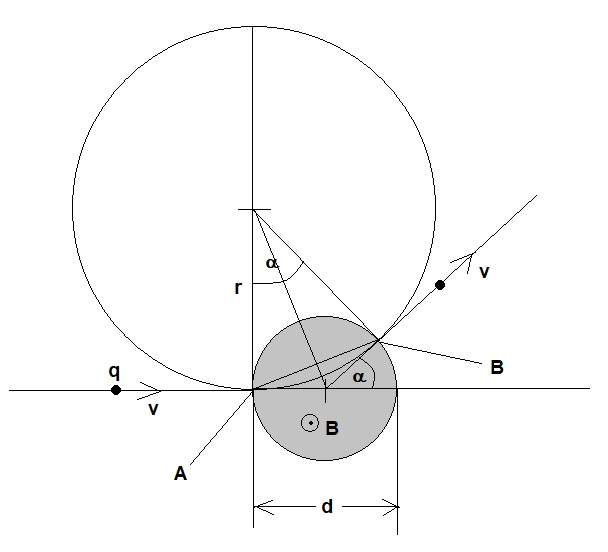
\includegraphics[width=.75\textwidth]{fig/elektronenstrahl-ablenkung_101.jpg}
    \caption{Skizze für Winkelberechnung (übernommen aus \cite{Blog})}
    \label{fig:ausBlog}
\end{figure}

\begin{figure}
    \centering
    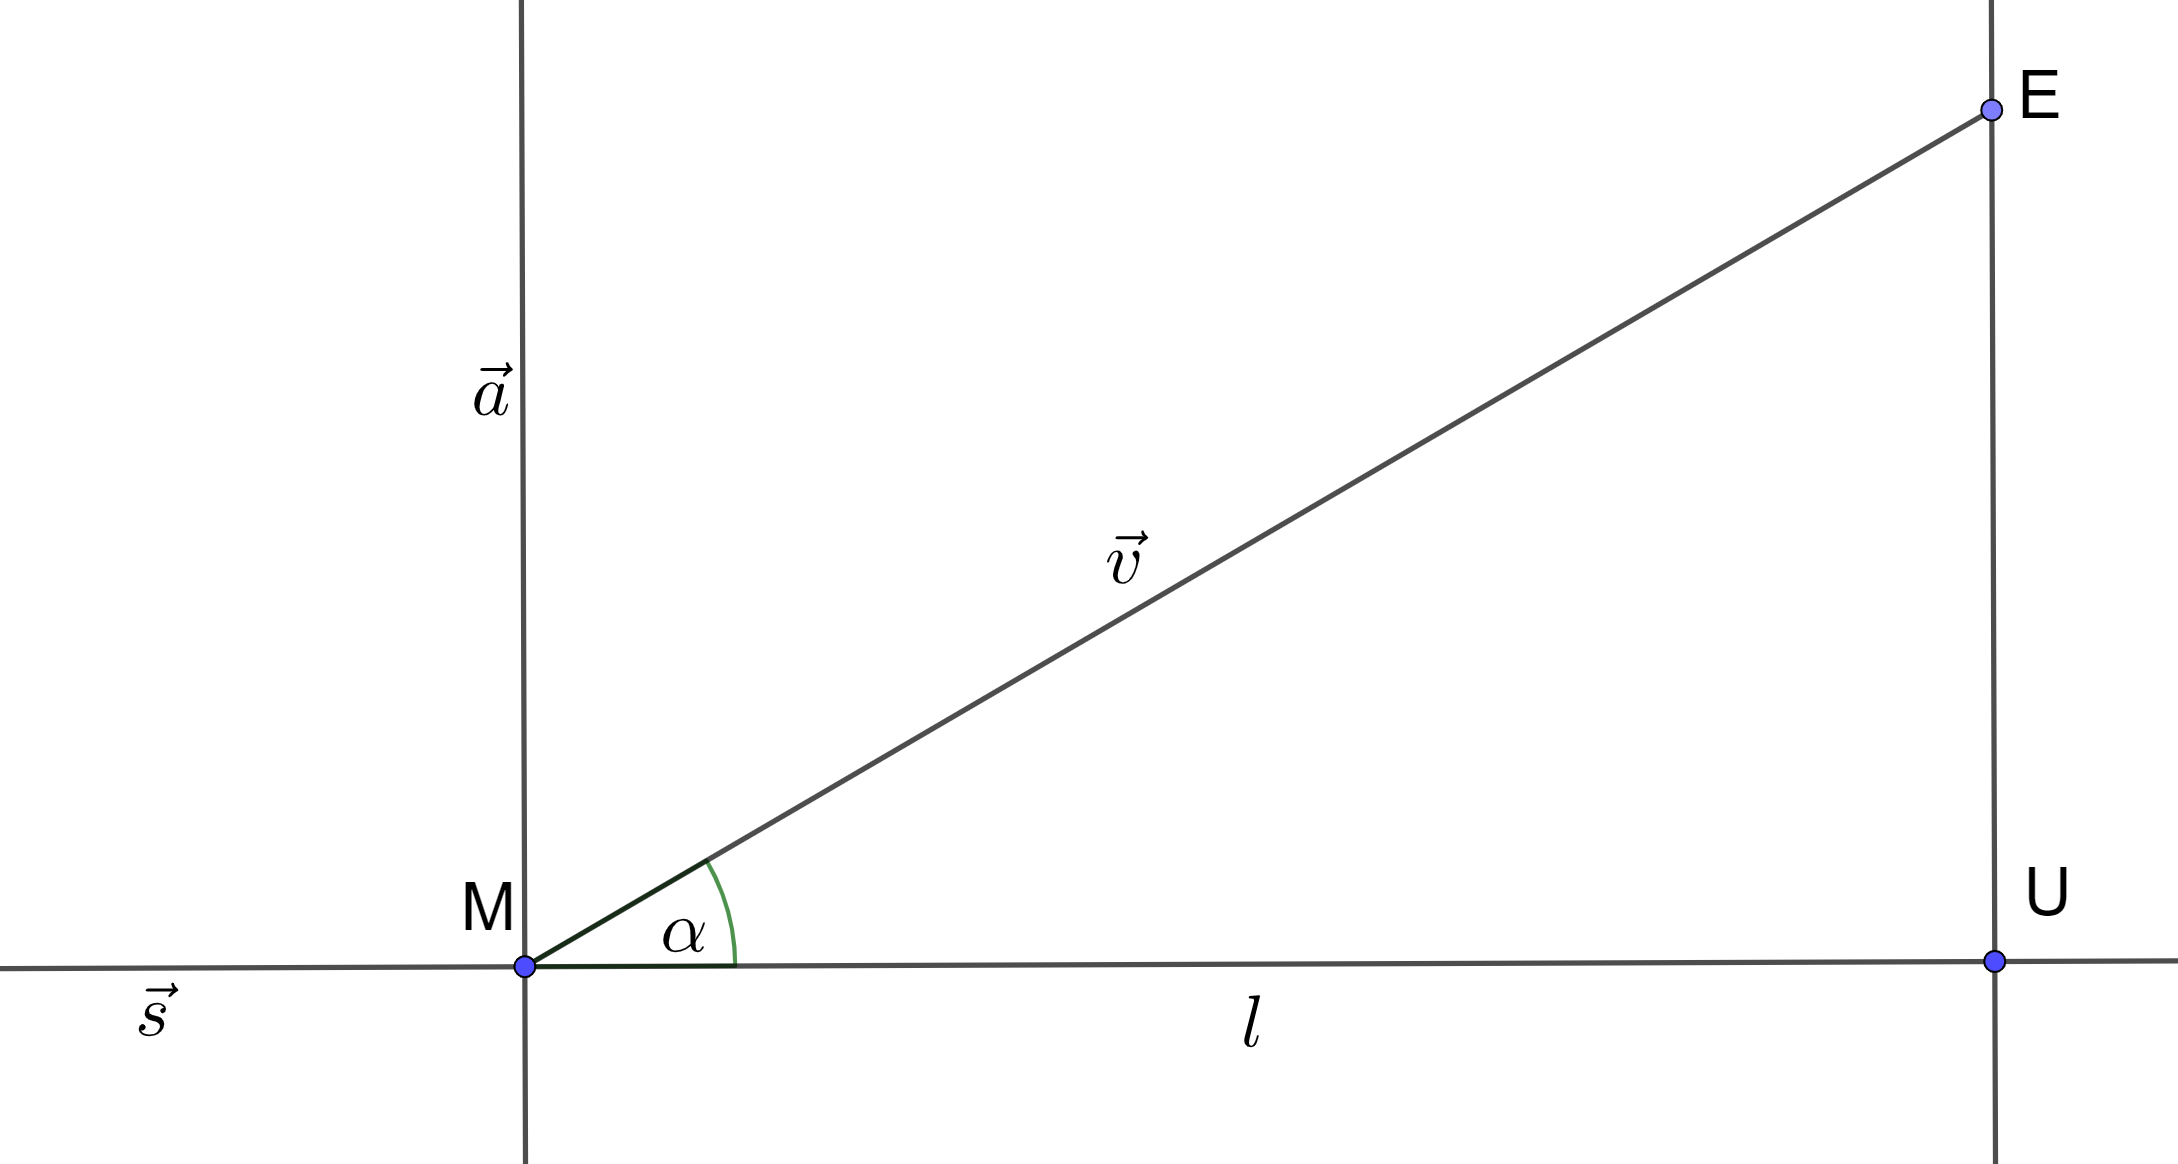
\includegraphics[width=.75\textwidth]{fig/Bildschirm_Skizze.png}
    \caption{Skizze für Auftreffen auf Bildschirm (mit GeoGebra erzeugt)}
    \label{fig:Schirm}
\end{figure}

%\subsection{Die geometrische Formel:}
\begin{equation}
    \label{eq:tan}
    \tan(\frac{\alpha}{2}) = \frac{d}{2}:r = \frac{d}{2 \cdot r}
\end{equation}

\begin{equation}
    \label{eq:a}
    \vv{a} = \vv{s} \cdot (-1) \times \vv{b}
\end{equation}

\begin{equation}
    \label{eq:v}
    \vv{v_\mathit{diff}} =  \vv{a} \cdot l \cdot \tan(\alpha)
\end{equation}

\subsection{Erklärung/Umsetzung der Physik im Code:}

Bei der Berechnung des Winkels $\alpha$ wird der arctans der oben bereits genannten Formel (\ref{eq:tan}) genommen und mit zwei multipliziert, da auf der Ausgabe der tatsächliche Winkel $\alpha$ zu sehen sein soll.
Der Winkel $\alpha$ wird im Bogenmaß berechnet.
Bei der \lstinline$Ablenkungsrichtung$ wird der Richtungsvektor des Strahl mit $-1$ multipliziert und danach das Kreuzprodukt mit dem Richtungsvektor des Ablenkspulenpaars genommen, wie bereits in Formel (\ref{eq:a}) genannt.
Durch den Befehl \lstinline$this.richtungsvektor$ wird auf den Richtungsvektor des jeweiligen Magnetfeldes verwiesen.
Des Weiteren ist noch hinzuzufügen, dass die Berechnung jedes Ablenkspulenpaar für sich macht und daher auch eigene Werte für \lstinline$alpha$, den \lstinline$Bahnradius$ und die \lstinline$Ablenkungsrichtung$ hat.
Der \lstinline$Ergebnisvektor$ ist ein Vektor, der gespeichert wird und später dafür verwendet wird, dass der Strahl vom Magneten zu dem Vektor auf dem Bildschirm gezeichnet wird.
Durch den \lstinline$for$- Befehl wird bewirkt, dass wie oben bereits genannt die Berechnung des \lstinline$Ergebnisvektors$ für jeden der Magneten gemacht wird.
Dies bedeutet, dass auf den \lstinline$Ergebnisvektor$, welcher zu Beginn auf den \lstinline$bildschirmabstand$ als x- Koordinate, $0$ als y-Koordinate und 0 als z-Koordinate gesetzt ist, erst die Formel (\ref{eq:v}9 benutzt wird und addiert wird.
Danach wird die Formel (\ref{eq:v}) erneut benutzt und erneut addiert. Dies führt dazu, dass der Punkt auf dem Schirm $E$ nun berechnet ist.

\begin{lstlisting}
alpha = 2 * Math.atan(felddurchmesser/ (2 *bahnradius ));
ablenkungsrichtung
  = strahl.quelle.richtungsvektor.
    multiplizieren(-1).
    kreuzprodukt(this.richtungsvektor);

Vektor ergebnisvektor = new Vektor(bildschirmabstand,0,0);
    for(Ablenkspulenpaar m : getWorld().getObjects(Ablenkspulenpaar.class) )
    {
        ergebnisvektor 
        = ergebnisvektor.addieren( m.ablenkungsrichtung.
        multiplizieren(bildschirmabstand*Math.tan(m.alpha)));
    }
return ergebnisvektor;

\end{lstlisting}

%\begin{tabular}{c|c|c}
    % Formel Buch & Formel Block & Anmerkungen  \\
     %\hline
    %$\alpha = \frac{d}{r}$ &$\tan(\frac{\alpha}{2}) = \frac{d}{2\cdot r}$& wegen Kleinwinkelnäherung bei dem Buch \\
    %\hline
   %$r = \frac{m\cdot v}{q\cdot B}$  & $r = \frac{m\cdot v}{q\cdot B}$& alles gleich 
     
%\end{tabular}



    \chapter{Polarlichter}
    \label{chap:polar}
    \section{Entstehung}%allgemein bleiben nicht auf gase und etc eingehen 
\section{Arten}%Bilder von Polarlichter wo von es abhängt% usage: \emptychapter[page displayed
                                        %        in toc]{name of the chapter}



    \chapter{Fazit}
    \label{chap:Fazit}
    



    % appendix for more or less interesting calculations
    \Appendix
    \chapter*{\appendixname} \addcontentsline{toc}{chapter}{\appendixname}
    % to make the appendix appear in ToC without number. \appendixname = 
    % Appendix or Anhang (depending on chosen language)
    \section{First Appendix Section}
Wonderful Appendix!

\lipsum[1-5]
 %\cleardoublepage



    % Bibliography
    \TheBibliography

    % BIBTEX
    % use if you want citations to appear even if they are not referenced to: 
    % \nocite{*} or maybe \nocite{Kon64,And59} for specific entries
    %\nocite{*}
    \bibliographystyle{babalpha}
    \bibliography{lit.bib}

    % THEBIBLIOGRAPHY
    %\begin{thebibliography}{000}
    %    \bibitem{ident}Entry into Bibliography.
    %\end{thebibliography}
\end{document}
